\documentclass{article}
\usepackage{amsmath}
\usepackage[margin=0.5in]{geometry}
\usepackage{breakcites}
\usepackage{natbib}
\usepackage{mathtools}
\usepackage{mathrsfs}
\usepackage{graphicx}
\usepackage{caption}
\usepackage{subcaption}
\usepackage[bottom]{footmisc}
\usepackage[export]{adjustbox}
\usepackage{todonotes}
\usepackage{footnote}
\usepackage{threeparttable}
\usepackage{booktabs}
\usepackage{multirow}
\usepackage{xspace}
\usepackage{siunitx}
% \usepackage{xr}
\usepackage{xr-hyper}
\usepackage{hyperref}
\hypersetup{
    colorlinks=true,
    linkcolor=blue,
    filecolor=magenta,
    urlcolor=cyan,
    citecolor=darkgray
}
\urlstyle{same}
\usepackage{newfloat}
\DeclareFloatingEnvironment[placement={!ht},name=List]{ordlist}

\DeclarePairedDelimiter\ceil{\lceil}{\rceil}
\DeclarePairedDelimiter\floor{\lfloor}{\rfloor}
\DeclareMathAlphabet\mathbfcal{OMS}{cmsy}{b}{n}
\DeclareMathOperator*{\argmin}{arg\,min}


\newcommand{\monosaccharide}[1]{{\bf #1}\xspace}
\newcommand{\nglycan}[0]{\textit{N}-glycan\xspace}
\newcommand{\nglycans}[0]{\textit{N}-glycans\xspace}

\newcommand{\msn}[0]{$MS^n$}

% Sample Name Shortcuts
\newcommand{\agp}[0]{\textit{20150930-06-AGP}\xspace}
\newcommand{\phil}[0]{\textit{20141031-07-Phil-82}\xspace}
\newcommand{\philbs}[0]{\textit{20141103-02-Phil-BS}\xspace}
\newcommand{\igg}[0]{\textit{20151002-02-IGG}\xspace}
\newcommand{\dpphil}[0]{\textit{20141128-11-Phil-82}\xspace}
\newcommand{\dpagp}[0]{\textit{AGP-DR-Perm-glycans-1}\xspace}
\newcommand{\rpagp}[0]{\textit{AGP-permethylated-2ul-inj-55-SLens}\xspace}
\newcommand{\rphumanserum}[0]{\textit{Perm-BS-070111-04-Serum}\xspace}
\newcommand{\rpserum}[0]{\textit{Perm-BS-070111-04-Serum}\xspace}

\newcommand{\reviewfootnote}[1]{\footnote{#1}}

\externaldocument[P-]{draft}[draft.pdf]
\begin{document}

\tableofcontents

\section{Chromatographic Feature Evaluation}\label{sec:feature_evaluation}
    For each candidate feature, we computed several statistics to estimate how distinguishable
    the observed signal was from random noise. We use the following quantities from each LC-MS
    feature:

    \renewcommand{\arraystretch}{1.5}
    \begin{table}
        \caption{Chromatogram Feature Definitions}\label{tbl:chromatogram_feature_definitions}
        \centering
        \begin{tabular}{l | p{9cm}}
            \hline
            $\mathcal{M}_i$ & The neutral mass of the $i$th chromatogram\\
            $\mathbfcal{I}_i$ & The total intensity array assigned to the $i$th chromatogram\\
            $\mathbfcal{I}_{i, j}$ & The sum of all peak intensities for peaks observed in
                                             the $j$th scan for the $i$th chromatogram\\
            $\mathcal{I}_{i, j, k}$ & The intensity assigned to the $k$th peak at the $j$th
                                      scan for the $i$th chromatogram\\
            $\mathbf{c}_i$ & The set of charge states observed for the $i$th chromatogram\\
            $\mathbfcal{I}_{i, c=j}$ & The total intensity assigned to the $i$th chromatogram
                                     with charge state $j$\\
            $\mathbf{t}_{i, j}$ & The time of the $j$th scan of the $i$th chromatogram\\
            $\textbf{env}_{i, j, k}$ & The normalized experimental isotopic envelope composing
                                     the $k$th peak of the $j$th scan of the $i$th chromatogram,
                                     whose members sum to $1$\\
            $\mathbf{a}_i$ & The set of adduction states observed for the $i$th chromatogram\\
            $\mathbfcal{I}_{i, a=j}$ & The total intensity assigned to the $i$th
                                                 chromatogram with adduct $j$\\
            ${\hat g}_i$ & The glycan composition assigned to the $i$th chromatogram, or \O
                           \ if there was no matched glycan composition
        \end{tabular}
    \end{table}
    \renewcommand{\arraystretch}{1.0}

    \subsection{Chromatographic Peak Shape}
        An LC-MS elution profile should be composed of one or more peak-like components, each
        following a bi-Gaussian peak shape model (\cite{Yu2010}) or in less ideal chromatographic
        circumstances, a skewed Gaussian peak shape model. We fit these models using non-linear
        least squares (NLS). As measures of goodness of fit are not generally available for NLS,
        we use the following criterion:
        \begin{align}
            {\hat y_i} &= NLS(\mathbfcal{I}_i, \mathbf{t}_i) \nonumber\\
            e_{i, NLS} &= \mathbfcal{I}_i - {\hat y_i} \nonumber\\
            {\bar y_i} &= \mathbf{t}_i
                \left(
                    \left(
                        \mathbf{t}_i^t\mathbf{t}_i
                    \right)^{-1}\mathbf{t}_i\mathbfcal{I}_i
                \right)\nonumber\\
            e_{i, null} &= \mathbfcal{I}_i - {\bar y_i} \nonumber\\
            \mathscr{L}_i &= 1 - \frac{\sum{e_{i, NLS}^2}}{\sum{e_{i, null}^2}}
        \end{align}
        \noindent where line score describes how much the peak shape fit improves on a ordinary
        least squares regression linear model.

        We apply two competitive peak fitting strategies to address distorted, overlapping, or
        multimodal elution profiles. The first works iteratively by finding a best-matching peak
        shape using non-linear least squares, subtracting the fitted signal and checks if there is
        another peak with at least half as tall as the removed peak, if so repeating the process until
        no peak can be found, saving each peak model so constructed. The second approach starts
        by locating local minima between putative peaks, and partitioning the chromatogram into
        sub-groups which would are fit independently. This method generates a candidate list of
        minima, and selects the case which has the greatest difference between the minimum and its
        pair of maxima to split the feature at. The strategy which produces the maximum $\mathscr{L}_i$
        is chosen.

    \subsection{Composition Dependent Charge State Distribution}
        % Does this principle need a citation?
        As the number of monosaccharides composing a glycan increases, the number of possible sites
        for charge localization increases. Under normal conditions, we would expect to observe the
        same molecule in multiple charge states (\cite{Maxwell2012}). Which charge states are
        expected would depend upon the size of the molecule and it's constituent units'
        electronegativity. In it's native state, \monosaccharide{NeuAc}'s acidic group causes
        glycans with one or more \monosaccharide{NeuAc} to have a propensity for higher negative
        charge states (\cite{Varki2009}). To capture this relationship, we modeled the probability of
        observing a glycan composition for sialylated and unsialylated compositions separately. For
        permethylated glycans, charge is carried by protons or metallic cation adducts like sodium,
        the relationship between acidic monosaccharides and charge state propensities is weaker.

        \begin{align}
            m_i &= (\floor*{(\mathcal{M}_i / w) / 10} + 1) * 10 \nonumber\\
            \mathcal{H}_{i,j} &= \frac{
                \mathbfcal{I}_{i, c=j}}{\mathbfcal{I}_i} \nonumber\\
            P(c, m) &= |m|\sum_{m_i \in m} \mathcal{H}_{i, j} \nonumber\\
            \mathscr{C}_i &= \sum_{c_{i, j} \in \mathbf{c}_i}{P(c_{i, j}, m_i)}
        \end{align}

        \noindent where $w$ is the width of the mass bin divided by 10 and $P(c, m)$ is defined as
        part of the model estimation procedure.

        \begin{figure}
            \centering
            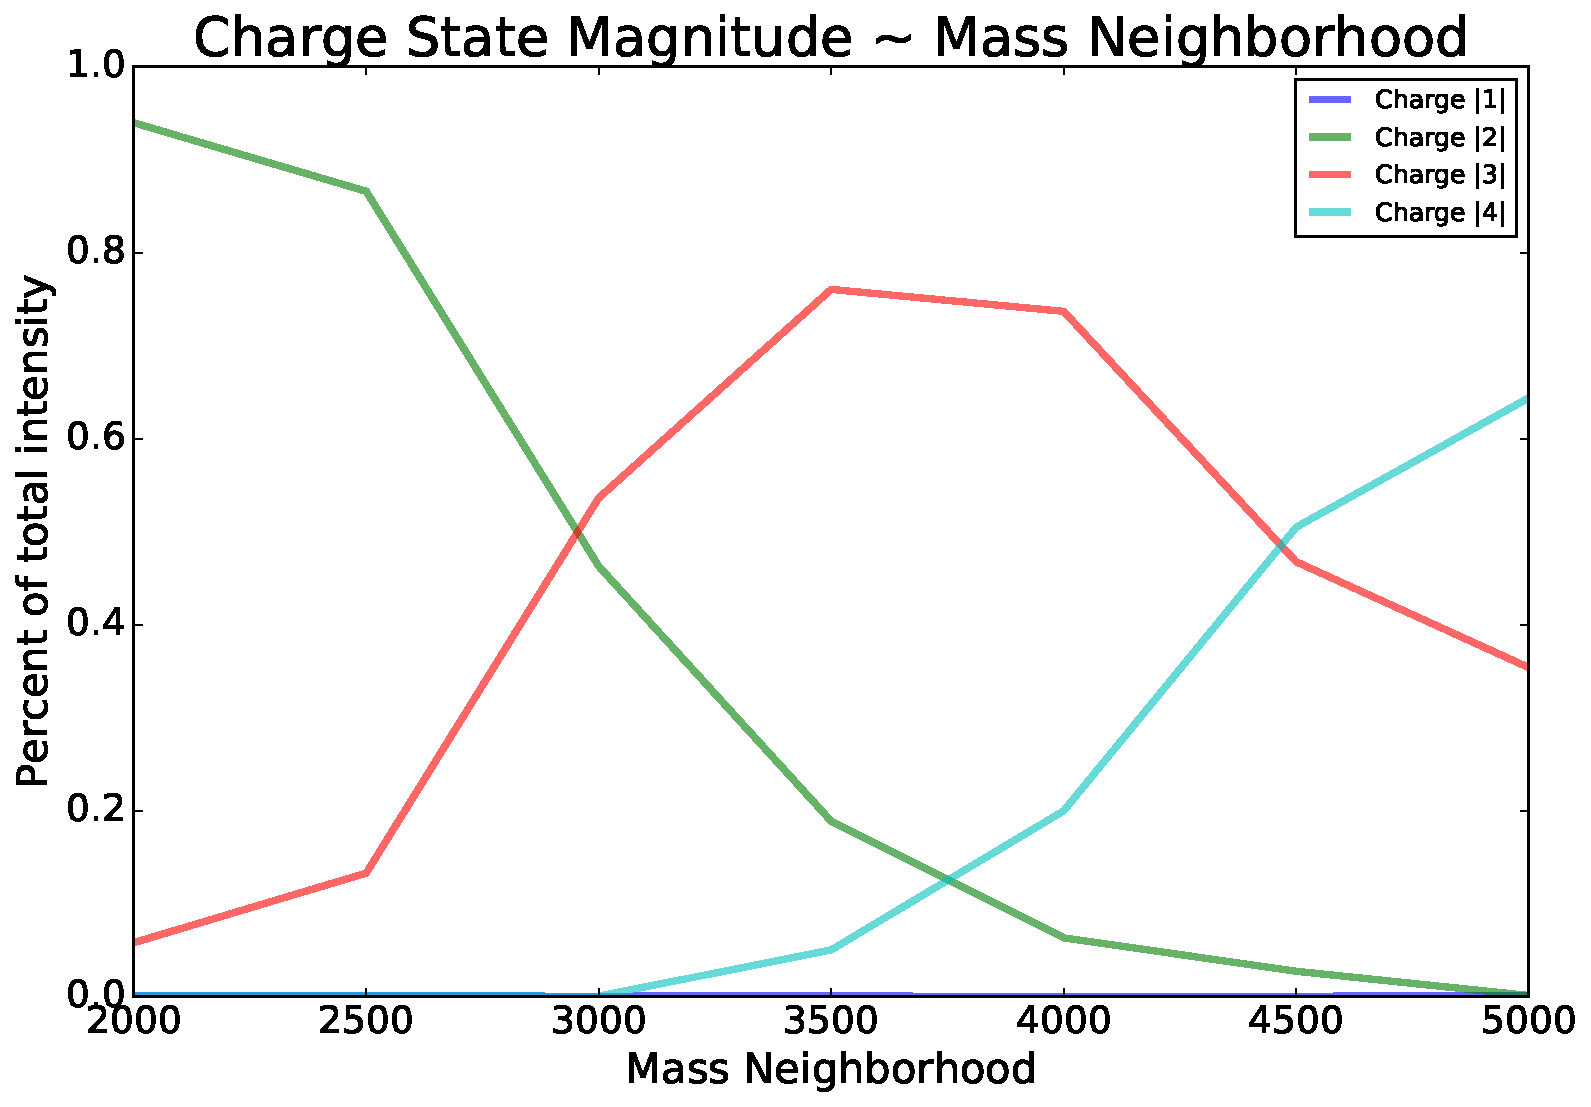
\includegraphics[width=0.75\linewidth]{figure/charge_trend_plot}
            \caption{The trend of charge state relative abundance for acidic glycans}
            \label{fig:charge_trend_plot}
        \end{figure}

    \subsection{Adduction Rate}
        For the samples \textit{AGP-permethylated-2ul-inj-55-SLens} and \textit{Perm-BS-070111-04-Human-Serum}
        we also include an Adduction Frequency model score $\mathscr{A}_i$, following the same
        pattern as the charge state distribution, with the same extension of justification
        from \cite{Maxwell2012}. We use one mass scaling model for all glycan compositions
        as ammmonium adduction is not expected to be composition dependent.

        \begin{align}
            \mathcal{H}_{i,j} &= \frac{
                \mathbfcal{I}_{i, a=j}}{\mathbfcal{I}_i} \nonumber\\
            P(a, m) &= |m|\sum_{m_i \in m} \mathcal{H}_{i, j} \nonumber\\
            \mathscr{A}_i &= \sum_{a_{i, j} \in \mathbf{a}_i}{P(a_{i, j}, m_i)}
        \end{align}

        We fit the adduction rate model on \textit{AGP-permethylated-2ul-inj-55-SLens} in order
        to make our comparison to third-party data less biased given limited sample data.

    \subsection{Isotopic Pattern Consistency}
        Our ahead-of-time deconvolution procedure uses an averagine isotopic model and does not
        capture the consistency of the isotopic pattern that was fit with the isotopic pattern
        of the glycan composition that matched that peak. The criterion
        \begin{align}
            \mathscr{I}_i &= 1 - 2\mathbfcal{I}_i^{-t}\mathbf{I}_i\sum_j^J{
                \sum_k^K{\mathcal{I}_{i, j, k}
                    \textbf{env}_{i, j, k}^t\left(
                        \ln{\textbf{env}}_{i, j, k} -
                        \ln{\textbf{tid}_{i}}
                    \right)
                }
            }
        \end{align}
        \noindent where \textbf{tid} is the theoretical isotopic pattern derived from either ${\hat g}_i$
        or an averagine interpolated for $\mathcal{M}_i$ if ${\hat g}_i =$ \O. This computes a
        per-peak intensity weighted mean G-test comparing the goodness of fit between the experimental
        envelope and the theoretical isotopic pattern.

    \subsection{Observation Spacing Score}
        The less time between observations of a glycan composition the less likely the chromatogram
        is to contain peaks missing or caused by isotopic pattern interference or missing information.
        \begin{align}
            \mathscr{T}_i &= 1 - 2\mathbfcal{I}_i^{-t}\mathbf{I}_i\sum_{j=1}^J\mathbfcal{I}_{i, j}(
                \mathbf{t}_{i, j} - \mathbf{t}_{i, j - 1})
        \end{align}

        As this feature depends heavily on the speed of the mass spectrometer, a scaling coefficient
        must be estimated from the data to reduce the penalty on slower instruments.

    \subsection{Summarization Score}
        Each scoring feature $\in \left[\mathscr{L}_i, \mathscr{C}_i, \mathscr{I}_i,
        \mathscr{T}_i\right]$ is penalized by $\epsilon = 1\mathrm{e}{-6}$ bounded in
        the range $[0, 1)$, with values below 0 set to $\epsilon$.

        \begin{align}
            s_i &= \sum_{f_{i,j} \in \text{features}_i}{\ln{
                \frac{f_{i, j}}{1 - f_{i, j}}
                }
            }
        \end{align}

        \noindent producing a value between $(-\infty, \infty)$. $s_i < 8$ reflects multiple
        poor feature scores and is unexpected to be real, while $s_i > 15$ is
        consistent with model expectations.


\section{A more complete derivation of ${\hat \phi}$}\label{sec:phi_hat_derivation}

    To obtain the optimal $\mathbf{\phi}$, we take the partial
        derivative of $\ell$ w.r.t $\phi_m$

        \begin{align}
            0 &= \frac{\partial\ell}{\partial\phi_m}\left((\mathbf{s} - \mathbf{\phi_o})^t(\mathbf{s} - \mathbf{\phi_o}) + \lambda
                \begin{bmatrix}
                    \phi_o - \tau_o, & \phi_m - \tau_m
                \end{bmatrix}
                \begin{bmatrix}
                    \mathbf{L_{oo}} & \mathbf{L_{om}} \\ \mathbf{L_{mo}} & \mathbf{L_{mm}}
                \end{bmatrix}
                \begin{bmatrix}
                    \phi_o - \tau_o \\ \phi_m - \tau_m
                \end{bmatrix}\right)\\
            &= \lambda(\phi_o - \tau_o)^t\mathbf{L_{om}} + \lambda\mathbf{L_{mo}}(\phi_o - \tau_o)
                 + \lambda(\phi_m - \tau_m)^t(\mathbf{L_{mm}}^t+ \mathbf{L_{mm}}) \nonumber\\
            &= 2\lambda\mathbf{L_{mo}}(\phi_o - \tau_o) + 2\lambda\mathbf{L_{mm}}(
                \phi_m - \tau_m) \nonumber\\
            -\mathbf{L_{mm}}(\phi_m - \tau_m) &= \mathbf{L_{mo}}(\phi_o - \tau_o) \nonumber\\
            (\phi_m - \tau_m) &= -\mathbf{L_{mm}}^{-1}\mathbf{L_{mo}}(\phi_o - \tau_o) \nonumber\\
            {\hat \phi_m} &= -\mathbf{L_{mm}}^{-1}\mathbf{L_{mo}}(\phi_o - \tau_o) + \tau_m
            \label{eqn:estimate_of_phi_m_complete}
        \end{align}

        \noindent and w.r.t. $\phi_o$

        \begin{align}
            0 &= \frac{\partial\ell}{\partial\phi_o}\left((\mathbf{s} - \mathbf{\phi_o}
                )^t(\mathbf{s} - \mathbf{\phi_o}) + \lambda
                \begin{bmatrix}
                    \phi_o - \tau_o, & \phi_m - \tau_m
                \end{bmatrix}
                \begin{bmatrix}
                    \mathbf{L_{oo}} & \mathbf{L_{om}} \\ \mathbf{L_{mo}} & \mathbf{L_{mm}}
                \end{bmatrix}
                \begin{bmatrix}
                    \phi_o - \tau_o \\ \phi_m - \tau_m
                \end{bmatrix}\right)\\
            &= -2\mathbf{s} + 2\phi_o +\lambda\left(\mathbf{L_{oo}} + \mathbf{L_{oo}}^t\right)(
                \phi_o - \tau_o) + \lambda\mathbf{L_{om}}(\phi_m - \tau_m) + \lambda\mathbf{
                L_{mo}}^t(\phi_m - \tau_m) \nonumber\\
            &= -2\mathbf{s} + 2\phi_o + 2\lambda\mathbf{L_{oo}}( \phi_o - \tau_o) + 2\lambda
                \mathbf{L_{om}}(\phi_m - \tau_m) \nonumber\\
            \mathbf{s} &= \phi_o + \lambda\left(\mathbf{L_{oo}}( \phi_o - \tau_o) +
                \mathbf{L_{om}}(\phi_m - \tau_m)\right) \nonumber\\
            &= \phi_o + \lambda\left(\mathbf{L_{oo}}( \phi_o - \tau_o) +
                \mathbf{L_{om}}(-\mathbf{L_{mm}}^{-1}\mathbf{L_{mo}}(
                \phi_o - \tau_o) + \tau_m - \tau_m)\right) \nonumber\\
            &= \phi_o + \lambda\left(\mathbf{L_{oo}}(\phi_o - \tau_o) -
                \mathbf{L_{om}}\mathbf{L_{mm}^{-1}}\mathbf{L_{mo}}(\phi_o - \tau_o)
                \right) \nonumber\\
            \mathbf{s} - \tau_o &= \phi_o - \tau_o + \lambda\left(\mathbf{L_{oo}}(\phi_o - \tau_o) -
                \mathbf{L_{om}}\mathbf{L_{mm}^{-1}}\mathbf{L_{mo}}(\phi_o - \tau_o)
                \right) \nonumber\\
            &= \mathbf{I}(\phi_o - \tau_o) + \lambda\left(\mathbf{L_{oo}}(\phi_o - \tau_o) -
                \mathbf{L_{om}}\mathbf{L_{mm}^{-1}}\mathbf{L_{mo}}(\phi_o - \tau_o)
                \right) \nonumber\\
            &= \left[
                \mathbf{I} + \lambda\left(\mathbf{L_{oo}} -
                    \mathbf{L_{om}}\mathbf{L_{mm}^{-1}}\mathbf{L_{mo}}
                \right)
            \right](\phi_o - \tau_o) \nonumber\\
            (\phi_o - \tau_o) &= \left[
                \mathbf{I} + \lambda\left(\mathbf{L_{oo}} -
                    \mathbf{L_{om}}\mathbf{L_{mm}^{-1}}\mathbf{L_{mo}}
                \right)
            \right]^{-1}(\mathbf{s} - \tau_o) \nonumber\\
            {\hat \phi_o} &= \left[
                \mathbf{I} + \lambda\left(\mathbf{L_{oo}} -
                    \mathbf{L_{om}}\mathbf{L_{mm}^{-1}}\mathbf{L_{mo}}
                \right)
            \right]^{-1}(\mathbf{s} - \tau_o) + \tau_o
            \label{eqn:estimate_of_phi_o_complete}
        \end{align}


\section{Estimation of Laplacian Regularization Parameters}\label{sec:laplacian_regularization_parameter_estimation}
    We model the relationship between $\mathbf{s}$, $\mathbf{\phi_o}$, and
    $\mathbf{\tau}$ as a set of gaussian distribution.
    \begin{align}
        \left(\mathbf{s}|\mathbf{\phi_o}, \mathbf{\tau}\right) &\sim
            \mathcal{N}(\mathbf{\phi_o}, \Sigma)\\
        \Sigma &= \rho\mathbf{I}
    \end{align}
    \begin{align}
        \left(\begin{bmatrix}
            \mathbf{\phi_o}\\
            \mathbf{\phi_m}
        \end{bmatrix}\middle|\mathbf{\tau}\right) &\sim
            \mathcal{N}(\mathbf{A\tau}, \lambda^{-1}\mathbf{L}^-)\\
        \left(\mathbf{\phi_o}\middle|\mathbf{\tau}\right) &\sim
            \mathcal{N}\left(\mathbf{A_o}\mathbf{\tau}, \Sigma_{\phi_o}\right)\\
        \Sigma_{\phi_o} &= \lambda^{-1}\left(
            \mathbf{L_{oo}} - \mathbf{L_{om}L_{mm}^{-1}L_{mo}}\right)^{-1}\\
        \mathbf{\tau} &\sim \mathcal{N}\left(0, \sigma^2\mathbf{I}\right)
    \end{align}

    \noindent Fully expanded, this becomes
    \begin{equation}
        \begin{bmatrix}
            \mathbf{s}\\
            \mathbf{\phi_o}\\
            \mathbf{\tau}
        \end{bmatrix} \sim \mathcal{N}\left(
            \begin{bmatrix}0\\0\\0\end{bmatrix},
            \begin{bmatrix}
                \Sigma + \Sigma_{\phi_o} + \sigma^2\mathbf{A_oA_o}^t &
                \Sigma_{\phi_o} + \sigma^2\mathbf{A_oA_o}^t &
                \sigma^2\mathbf{A_o}\\
                \Sigma_{\phi_o} + \sigma^2\mathbf{A_oA_o}^t &
                \Sigma_{\phi_o} + \sigma^2\mathbf{A_oA_o}^t &
                \sigma^2\mathbf{A_o}\\
                \sigma^2\mathbf{A_o}^t & \sigma^2\mathbf{A_o}^t & \sigma^2\mathbf{I}\\
            \end{bmatrix}
        \right)\label{eqn:multivariate_gaussian_model}
    \end{equation}

    We can form the conditional distribution $\tau|\mathbf{s}$ which has a mean

    \begin{align}
        \mu_{\tau|\mathbf{s}} &= 0 + (\sigma^2\mathbf{A_o}^t)\left(
            \Sigma + \Sigma_{\phi_o} + \sigma^2\mathbf{A_oA_o^t}\right)^{-1}\mathbf{s}\\
        % &= \mathbf{A_o}^t\left(
        %     \frac{\rho}{\sigma^2}\mathbf{I} + \frac{1}{\lambda\sigma^2}\mathbf{L_{oo}^-} + 
        %     \mathbf{A_oA_o^t}
        %     \right)^{-1}\mathbf{s} \nonumber\\
        &= \mathbf{A_o}^t\left(
            {\tilde\rho}\mathbf{I} + \frac{1}{{\tilde\lambda}}\mathbf{L_{oo}^-} + 
            \mathbf{A_oA_o^t}
            \right)^{-1}\mathbf{s} \label{eqn:tau_given_s}
    \end{align}

        We assume that $\sigma^2 \gg 1$, and treat $\lambda$ and $\rho$
    as relative to $\sigma^2$, as ${\tilde \rho}$ and ${\tilde \lambda}$.
    This model gives us an estimate for $\tau$ given a value for
    $\rho$ and $\lambda$. As $\rho$ has no direct role in the central
    tendency of $\mathbf{\phi}$ or $\mathbf{s}$, we choose to fix the
    value of ${\tilde \rho} = 0.1$, which leaves only ${\tilde \lambda}$.
    We estimate the optimal ${\tilde \lambda}$ by grid search, minimizing
    the predicted residual error sum of squares (PRESS) statistic.

    \begin{align}
        \argmin_{\tilde \lambda} & \frac{\mathbf{s - {\hat \phi_o}}}{\left(
            1 - \left(
                \mathbf{I} + {\tilde \lambda}\mathbf{L}
            \right)^{-1}
        \right)^2}
    \end{align}

        This formulation depends upon the value of \textbf{s} and is
    sensitive to low scoring matches, which can lead to incorrect
    estimates of $\tau$ and PRESS. We therefore perform a grid
    search over both ${\tilde \lambda}$ and a minimum threshold
    for \textbf{s}, $\gamma$.

    % Does this network pruning merit a pseudo-code section?
        As we increase $\gamma$ we remodel the graph $\mathcal{G}$,
    removing nodes whose score is below $\gamma$. For each pair
    of neighbors of removed node $g_m$, $(g_u, g_v)$, if
    $L_1(g_u, g_v) >  L_1(g_u, g_m) + L_1(g_m, g_v)$, we add an
    edge from $g_u$ to $g_v$ with weight $\frac{1}{L_1(g_u, g_m)
    + L_1(g_m, g_v)}$, up to a limit of $L_1(g_k, g_m) < 5$.
    We give the result of this grid search the name $\mathbf{r}$.
    At each point, on the grid, we save the value of $\tau$ in
    $r_{\lambda_i, \gamma_j, \tau}$ and the PRESS in $r_{
    \lambda_i, \gamma_j, PRESS}$. To select the optimal parameters,
    we traverse the grid along $\gamma$, computing $\mathbf{\tau_\gamma}$:

    \begin{align}
        {\bar \lambda_j} &= \argmin_{\lambda_i}{r_{\lambda_i, \gamma_j, PRESS}} \\
        \tau_{\gamma_j} &= |r_{{\bar \lambda_j}, \gamma_j, \tau}| * \left(
            \frac{\gamma_j}{b} + (1 - \frac{1}{b})\right)
    \end{align}

    \noindent where $b$ is a bias factor defining how much
    weight to give to higher values of $\gamma$ which
    correspond to networks made up of higher confidence
    assignments. We chose $b = 4$. We define ${\bar \tau_\gamma} =
    \max{\mathbf{\tau_\gamma}}$ and define the  vector
    $\mathbf{\bar \gamma} = \left[\gamma_j \leftarrow\tau_{\gamma_j}
    \ge {\bar \tau_\gamma} * 0.95\right]$. This favors values of
    $\gamma$ where large values of $\tau$ are selected, meaning that
    the neighborhoods are well populated, while also giving an estimate
    for ${\tilde \lambda}$ that is non-zero. We term the values of
    $\gamma$ in $\mathbf{{\bar \gamma}}$ the {\em target thresholds}
    of \textbf{s}.

        To estimate ${\tilde \lambda}$ and $\tau$ from these results,
    we select the columns of the grid $\mathbf{r}$ at each $\gamma_j
    \in \mathbf{{\bar \gamma}}$ and applied the following procedure:

    \begin{align}
    % The maximum tau from the grid search over gamma
    {\bar \tau_\gamma} &= \max{\mathbf{\tau_\gamma}}\\
    % Those values of gamma whose tau is within 10% of the maximum value of tau
    % observed
    \mathbf{\bar \gamma} &= \left\{\gamma_j \leftarrow\tau_{\gamma_j}
        \ge {\bar \tau_\gamma} * 0.9\right\}\\
    % The PRESS minimizing lambda values assocaited with these selected gamma
    {\bar \lambda} &= \left\{ {\bar \lambda_j} \leftarrow \gamma_j \in {\bar \gamma}\right\}\\
    % The observed scores in the partitions which exceed the threshold gamma
    \mathbf{s_{\gamma_j}} &= \left\{s_i \leftarrow s_i > \gamma_j\right\} \\
    % The new estimated tau based upon the selected partion
    \mathbf{{\bar \tau_j}} &= \mu_{\tau|\mathbf{s}_{\gamma_j}, {\bar \lambda}_j}\\
    % The average selected lambda
    {\hat \lambda} &= \frac{1}{|\mathbf{{\bar \lambda}}|}\sum_j {\bar \lambda}_j\\
    % The average selected tau
    {\hat \tau} &= \frac{1}{|\mathbf{{\bar \tau}}|}\sum_j \mathbf{{\bar \tau_j}}\\
    % The average threshold gamma
    {\hat \gamma} &= \frac{1}{|\mathbf{{\bar \gamma}}|}\sum_j {\bar \gamma}_j
    \end{align}

    \noindent where $\mathbf{s}_{\gamma_j}$ is the set of observed
    scores which are greater than $\gamma_j$, but where the estimation
    of is carried out with the complete Laplacian $\mathbf{L}$,
    not the reduced network used to compute $\mathbf{r}$. This set of
    averaged estimates of ${\hat \lambda}$ and ${\hat \tau}$ are then
    used to estimate ${\hat \phi_o}$ by \ref{eqn:estimate_of_phi_o_complete}, labeled
    \ref{P-eqn:estimate_of_phi_o} in the main text.


\section{$MS^n$ Signature Ion Criterion}\label{sec:signature_ion_criterion}
    \textbf{This feature was not used in the main article in order to make the comparison
    between our results and previously published work more straight forward.}

    When \msn scans are present, it  may be useful to consider only those $MS^1$
    features which are associated with \msn scans that contain glycan-like signature
    ions. We include an algorithm for classifying an \msn scan as being "glycan-like":

    \begin{align}
        I &= max(intensity(p)) \\
        t &= I * 0.01 \\
        p_{oxonium} &= \{p_i \leftarrow |ppmerror(mass(p_j), mass(f_g))| < e,
                         f_g \in oxonium(g), f_g \ne \text{Fucose}, intensity(p_i) > t\}\\
        p_{edges} &= \{(p_i, p_j) \leftarrow |ppmerror(mass(p_j) - mass(p_i), mass(f_g))| < e,\\
                  &\phantom{{}=1} oxonium(f_g) \in g , intensity(p_i) > t, intensity(p_j) > t\} \notag\\
        s_{oxonium} &= \frac{1}{|p_{oxonium}|}\sum_{p_i}^{p_{oxonium}}{
                \left(\frac{intensity(p_i)}{I}\right)
            } * min(log_4|p_{oxonium}|, 1)\\
        s_{edges} &= \frac{1}{|p_{edges}|}\sum_{p_i, p_j}^{p_{edges}}{
                \left(\frac{intensity(p_i) + intensity(p_j)}{I}\right)
            } * min(log_4|p_{edges}|, 1)\\
        s_g &= max(s_{oxonium}, s_{edges})\\
    \end{align}

    Where $p$ is the set of peaks in the scan, $g$ is the glycan compostion, $e$ the
    required parts-per-million mass accuracy. $oxonium()$ is a function that given
    a glycan composition $g$, produces fragments $f_g$ of $g$ composed of between one
    and three monosaccharides, commonly observed as oxonium ions alone, or as the mass
    difference between two peaks formed from consecutive fragmentation of a glycosidic
    bond. This method is not intended to identify a glycan structure, just detect patterns in
    the signal peaks of the \msn scan that could indicate the fragmentation of a glycan.



\section{Algorithmic Performance on All Datasets}\label{sec:algorithm_performance}
    For more details on each sample, please see Table \ref{tab:sample_overview}.

\subsection{Results for AGP}
    
    We analyzed three different sample workups of \nglycans released from Alpha 1 Acid
    Glycoprotein. See Table~\ref{tab:agp_parameter_estimates} for a comparison of estimated $\tau$
    values for each sample. For \dpagp and \rpagp, we used an $MS^n$ Signature Ion Criterion
    threshold of 0.17 to filter out large contaminants that may be introduced by permethylation
    reagents.

    The estimate of $\gamma$ for \agp was larger than the score for the larger penta-antennary 

    \begin{table}[h]
        \centering
        \small
        \begin{tabular}{l SSS}
            \toprule
            $\tau_i$ & {\agp} & {\dpagp} & {\rpagp}\\
            \midrule
            high-mannose & 0.000 & 0.000 & 0.000\\
            hybrid & 11.520 & 7.240 & 21.092\\
            bi-antennary & 15.691 & 12.859 & 20.627\\
            asialo-bi-antennary & 0.000 & 0.000 & 13.253\\
            tri-antennary & 21.752 & 21.693 & 21.550\\
            asialo-tri-antennary & 0.000 & 0.000 & 6.792\\
            tetra-antennary & 15.993 & 15.276 & 17.452\\
            asialo-tetra-antennary & 0.000 & 0.000 & 0.000\\
            penta-antennary & 11.446 & 10.127 & 7.282\\
            asialo-penta-antennary & 0.000 & 0.000 & 0.000\\
            hexa-antennary & 2.211 & 0.000 & 0.000\\
            asialo-hexa-antennary & 0.000 & 0.000 & 0.000\\
            hepta-antennary & 0.000 & 0.000 & 0.000\\
            asialo-hepta-antennary & 0.000 & 0.000 & 0.000\\
            \midrule
            ${\hat \lambda}$ & 0.99 & 0.99 & 0.99\\
            ${\hat \gamma}$ & 15.74 & 16.22 & 17.64\\
            \bottomrule
        \end{tabular}
        \caption{Estimated values of smoothing parameters $\tau$, $\lambda$, and $\gamma$ for each
                 AGP-based dataset and using a combinatorial database \label{tab:agp_parameter_estimates}}
    \end{table}

    \begin{figure}[htb]
        \centering
        \begin{minipage}{1\linewidth}
            \centering
            \begin{subfigure}[b]{0.49\linewidth}
                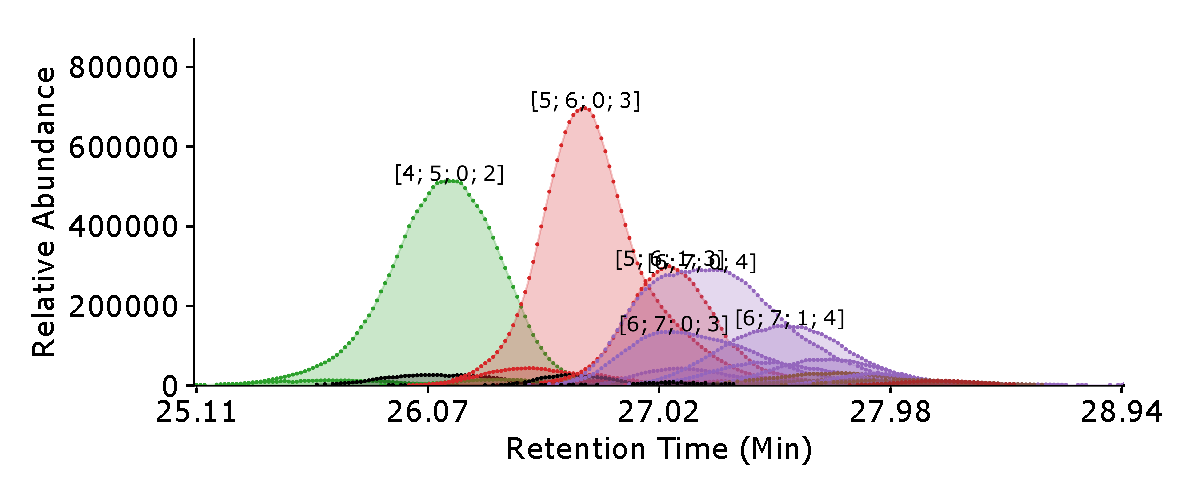
\includegraphics[width=1\linewidth, valign=t]{figure/native_agp_chromatograms.eps}
                \subcaption{
                    \label{fig:agp_assignment:a}
                }
            \end{subfigure}
            \vspace{0pt}
            \begin{subfigure}[b]{0.49\linewidth}
                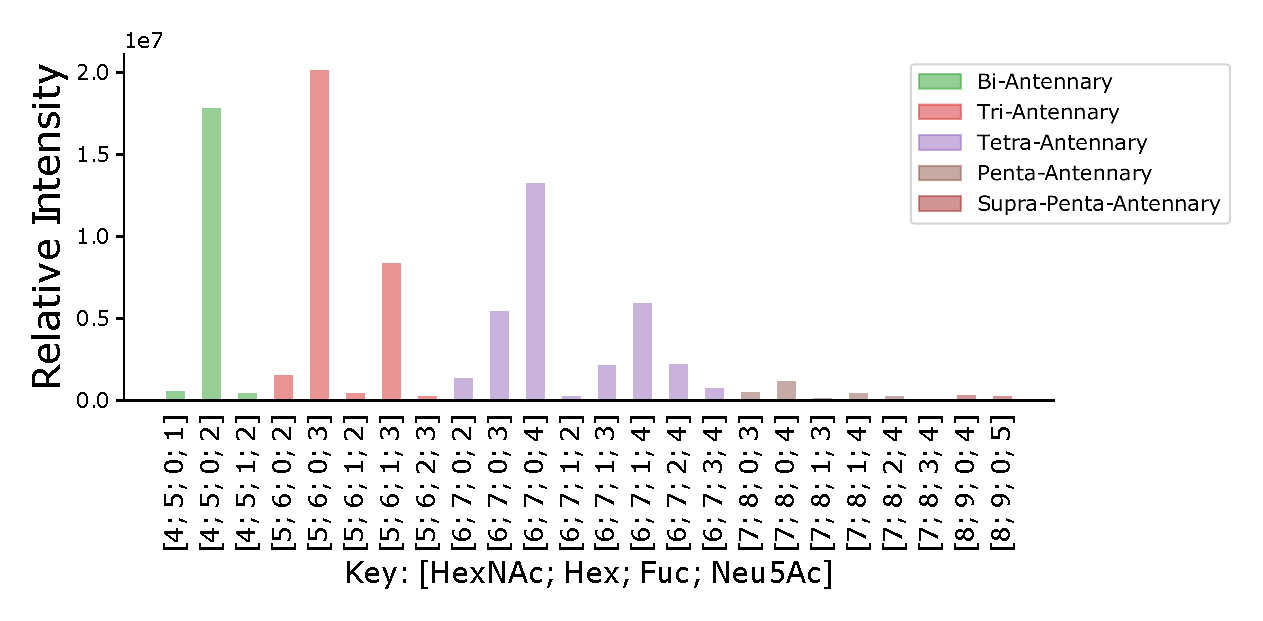
\includegraphics[width=1\linewidth, valign=b]{figure/native_agp_abundances.eps}
                \subcaption{
                    \label{fig:agp_assignment:b}
                }
            \end{subfigure}
        \end{minipage}
        \begin{minipage}{1\linewidth}
            \centering
            \begin{subfigure}[b]{0.49\linewidth}
                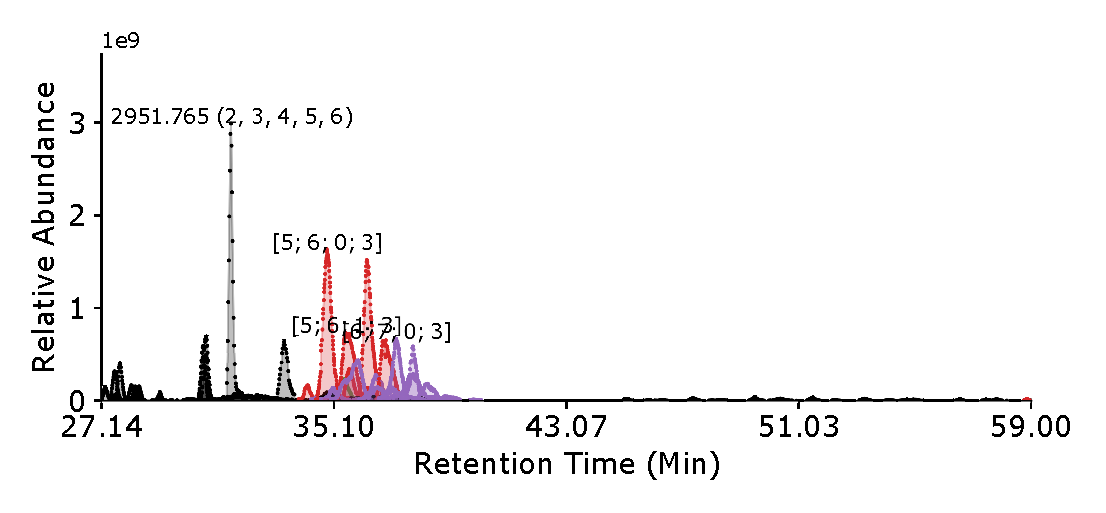
\includegraphics[width=1\linewidth, valign=t]{figure/dp_agp_chromatograms.eps}
                \subcaption{
                    \label{fig:agp_assignment:c}
                }
            \end{subfigure}
            \vspace{0pt}
            \begin{subfigure}[b]{0.49\linewidth}
                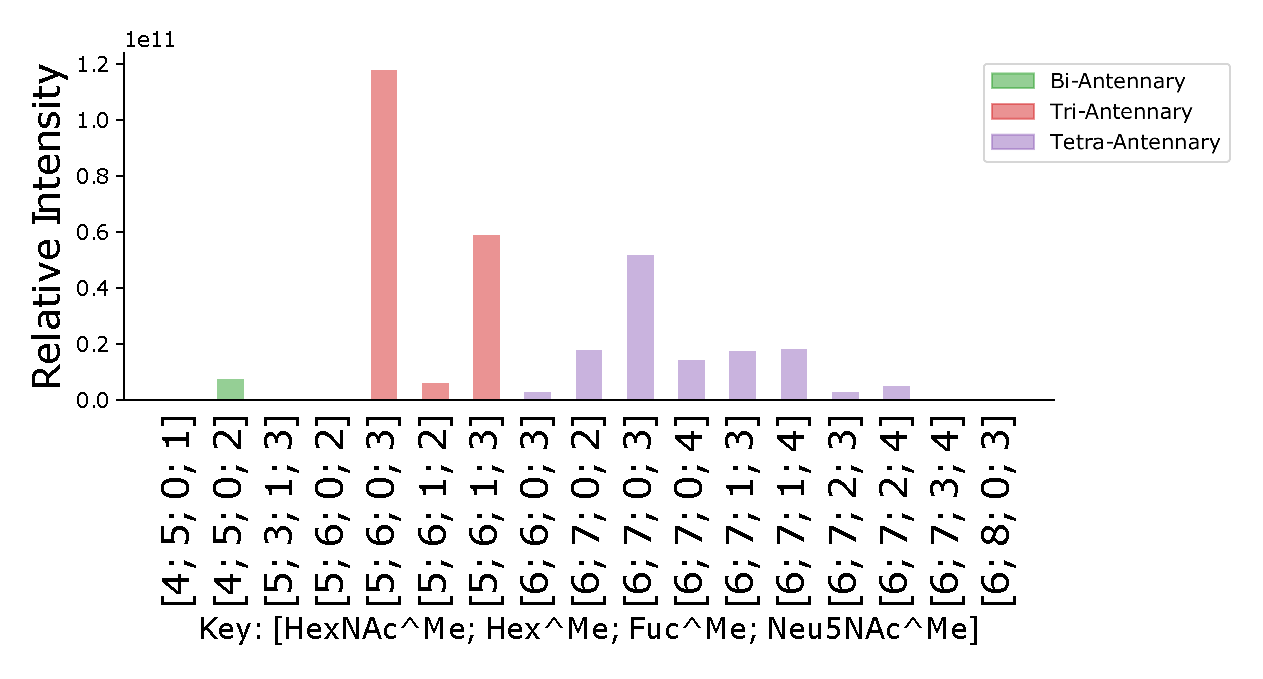
\includegraphics[width=1\linewidth, valign=b]{figure/dp_agp_abundances.eps}
                \subcaption{
                    \label{fig:agp_assignment:d}
                }
            \end{subfigure}
        \end{minipage}
        \begin{minipage}{1\linewidth}
            \centering
            \begin{subfigure}[b]{0.49\linewidth}
                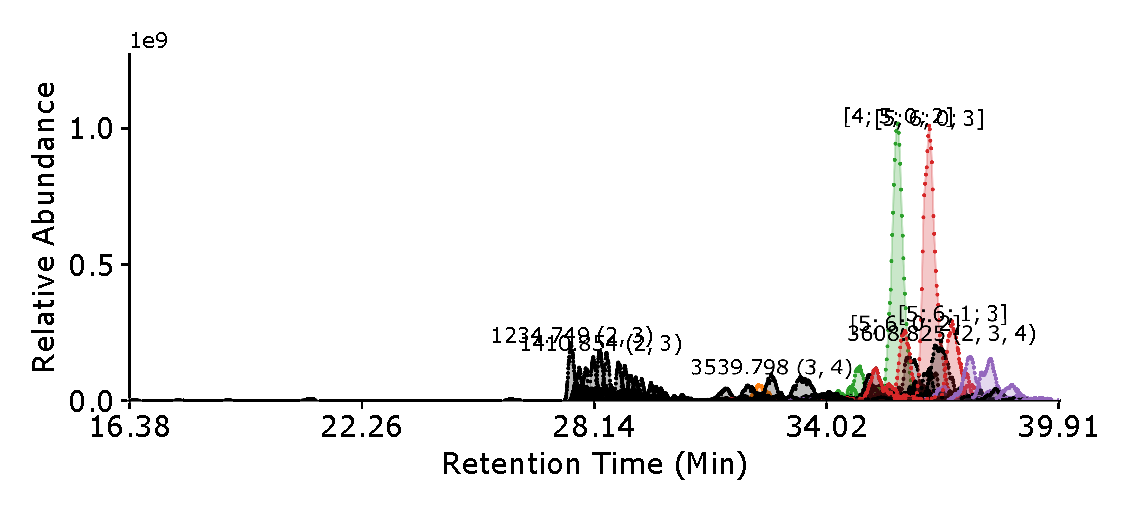
\includegraphics[width=1\linewidth, valign=t]{figure/rp_agp_chromatograms.eps}
                \subcaption{
                    \label{fig:agp_assignment:e}
                }
            \end{subfigure}
            \vspace{0pt}
            \begin{subfigure}[b]{0.49\linewidth}
                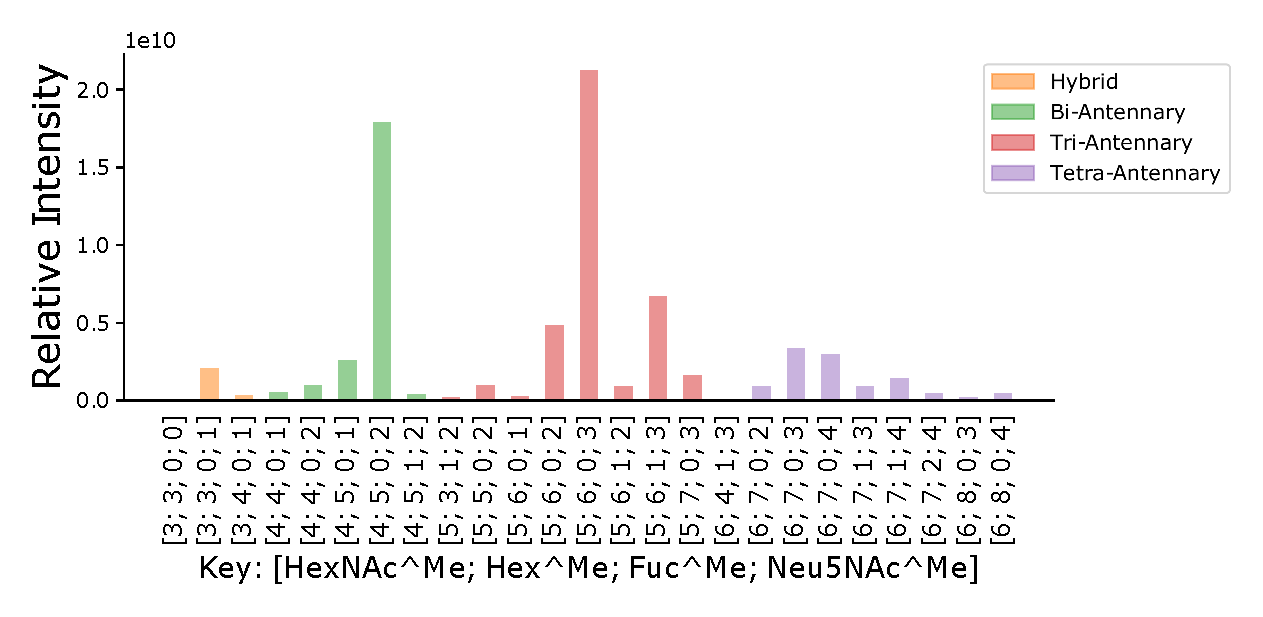
\includegraphics[width=1\linewidth, valign=b]{figure/rp_agp_abundances.eps}
                \subcaption{
                    \label{fig:agp_assignment:f}
                }
            \end{subfigure}
        \end{minipage}
        \caption{Chromatogram Assignments for \agp (a, b), \dpagp (c, d) and \rpagp (e, f)
            \label{fig:agp_assignments}
        }
    \end{figure}
    \FloatBarrier

\subsection{Results for Phil-82}

    We analyzed native and deutero-reduced and permethylated \nglycans released from
    virions of Influenza-A Virus strain Phillipines 1982, both samples acquired on a QTOF
    mass spectrometer. See Table~\ref{tab:phil82_parameter_estimates}
    for a comparison of estimated $\tau$ values for each sample. In the case of \dpphil,
    \msn scans were acquired, resulting in lower resolution chromatographic peaks. We observed
    little ammonium adduction in \dpphil. As expected, we observed abundant formate adduction in
    \phil, particularly on the high mannose glycans. \dpphil also displays considerable in-source
    fragmentation of the high mannose series, defined by the multimodal chromatographic peaks of
    smaller high mannose glycans appearing in lower abundance directly under larger peaks for
    high mannose glycans. This fragmentation, combined with permethylation altering the ionization
    efficiency of these analytes, makes a direct comparison of glycan composition abundance between
    \phil and \dpphil inadvisable. We observe markedly different peak shapes between \phil and \dpphil
    but the relative order of elution is preserved, with the largest high mannose glycans eluting
    later than the largest observed complex type.

    \begin{table}[h]
        \centering
        \small
        \begin{tabular}{l SS}
            \toprule
            $\tau_i$ & {\phil} & {\dpphil}\\
            \midrule
            high-mannose & 17.070 & 19.395\\
            hybrid & 14.039 & 17.147\\
            bi-antennary & 0.000 & 0.000\\
            asialo-bi-antennary & 16.287 & 17.689\\
            tri-antennary & 0.000 & 0.000\\
            asialo-tri-antennary & 15.220 & 18.865\\
            tetra-antennary & 0.000 & 0.000\\
            asialo-tetra-antennary & 7.103 & 7.660\\
            penta-antennary & 0.000 & 0.000\\
            

            asialo-penta-antennary & 0.000 & 3.365\\
            hexa-antennary & 0.000 & 0.000\\
            asialo-hexa-antennary & 0.000 & 0.000\\
            hepta-antennary & 0.000 & 0.000\\
            asialo-hepta-antennary & 0.000 & 0.000\\
            \midrule
            ${\hat \lambda}$ & 0.99 & 0.99\\
            ${\hat \gamma}$ & 16.51 & 15.50\\
            \bottomrule
        \end{tabular}
        \caption{Estimated values of smoothing parameters $\tau$, $\lambda$, and $\gamma$ for each
                 Phil-82-based dataset and using a combinatorial database \label{tab:phil82_parameter_estimates}}
    \end{table}

    \begin{figure}[tb]
        \centering
        \begin{minipage}{1\linewidth}
            \centering
            \begin{subfigure}[b]{0.49\linewidth}
                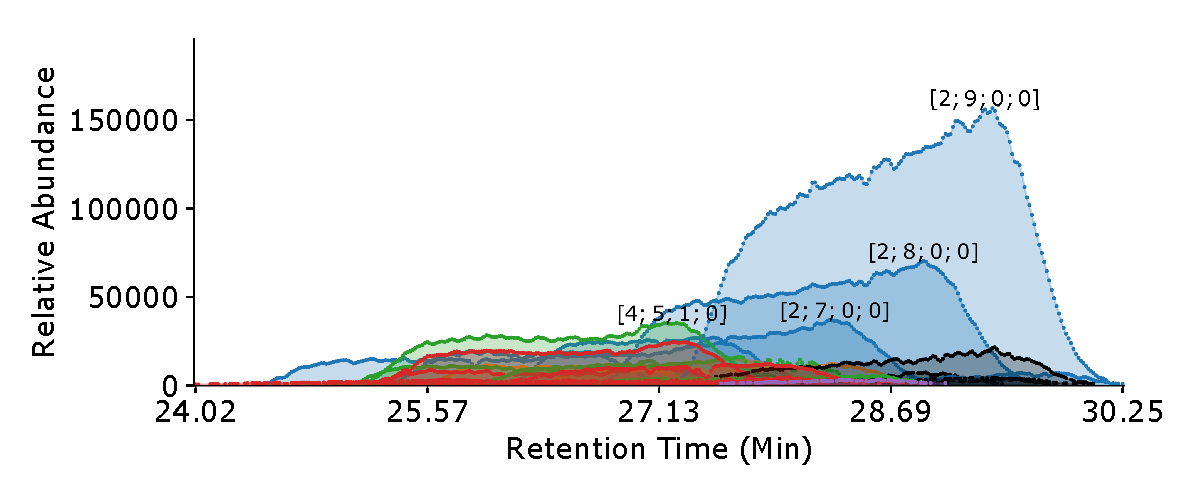
\includegraphics[width=1\linewidth, valign=t]{figure/native_phil82_chromatograms.eps}
                \subcaption{
                    \label{fig:phil82_assignment:a}
                }
            \end{subfigure}
            \vspace{0pt}
            \begin{subfigure}[b]{0.49\linewidth}
                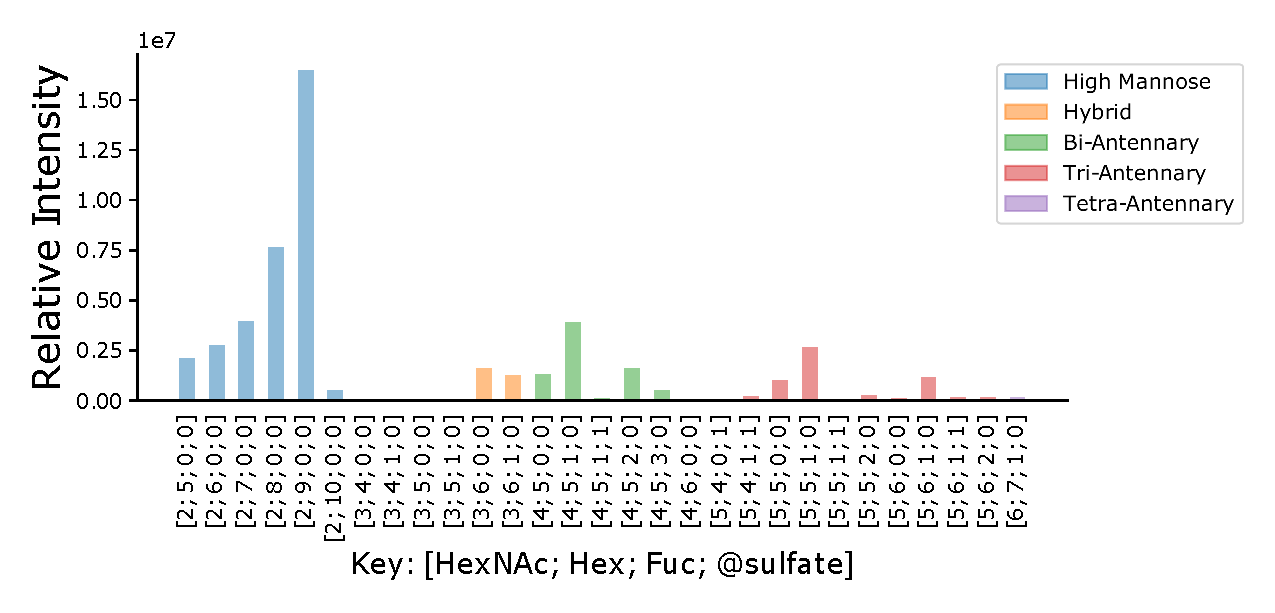
\includegraphics[width=1\linewidth, valign=b]{figure/native_phil82_abundances.eps}
                \subcaption{
                    \label{fig:phil82_assignment:b}
                }
            \end{subfigure}
        \end{minipage}
        \begin{minipage}{1\linewidth}
            \centering
            \begin{subfigure}[b]{0.49\linewidth}
                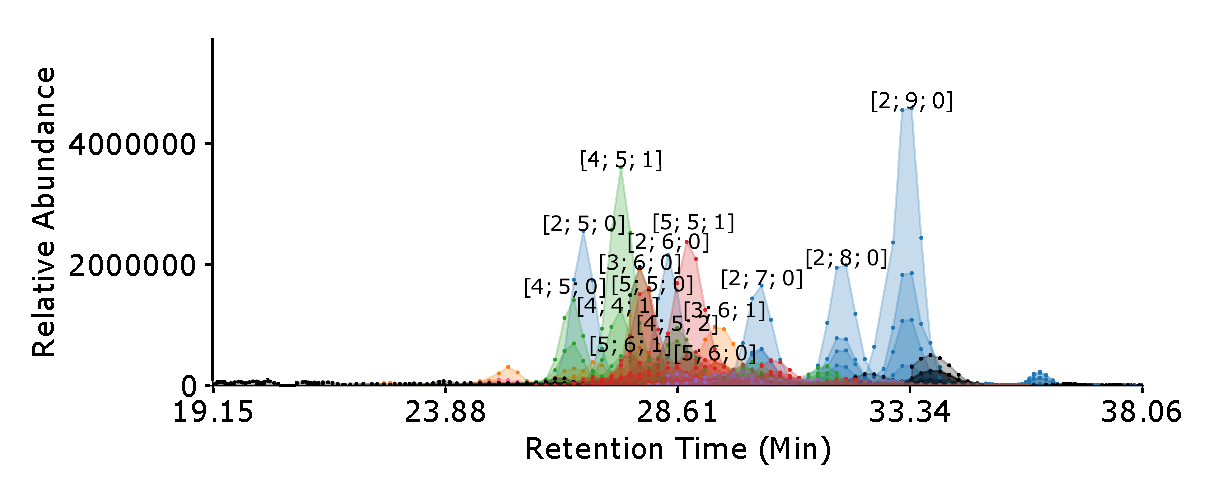
\includegraphics[width=1\linewidth, valign=t]{figure/dp_phil82_chromatograms.eps}
                \subcaption{
                    \label{fig:phil82_assignment:c}
                }
            \end{subfigure}
            \vspace{0pt}
            \begin{subfigure}[b]{0.49\linewidth}
                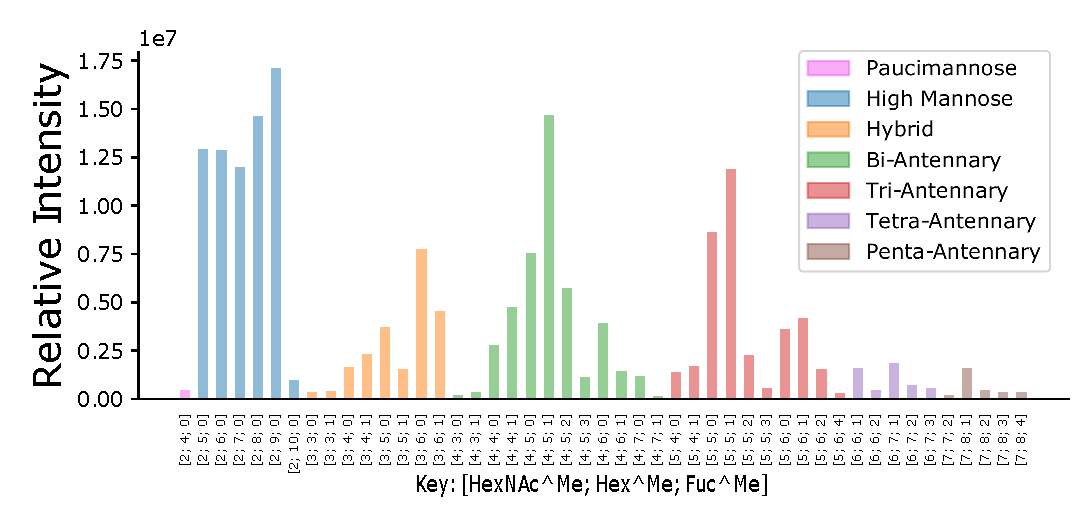
\includegraphics[width=1\linewidth, valign=b]{figure/dp_phil82_abundances.eps}
                \subcaption{
                    \label{fig:phil82_assignment:d}
                }
            \end{subfigure}
        \end{minipage}
        \caption{Chromatogram Assignments for \phil (a, b) and \dpphil (c, d)
            \label{fig:phil82_assignments}
        }
    \end{figure}

\FloatBarrier
\subsection{Results for IGG}
    We analyzed native \nglycans released from IgG. The estimated $\tau$ values shown in
    Table~\ref{tab:igg_parameter_estimates}are consistent with the expectation that IgG
    glycans will be either hybrid or small complex-type structures. These findings are
    consistent with the results from \citealp{Peltoniemi2013}, though their study used
    different sample preparation and instrumentation, and their data were not available
    for side-by-side comparison. The EICs and integrated abundances for this sample are
    shown in Figure~\ref{fig:igg_assignments}.
    
    \begin{table}[h]
        \centering
        \small
        \begin{tabular}{l S}
            \toprule
            $\tau_i$ & {\igg}\\
            \midrule
            high-mannose & 0.000\\
            hybrid & 15.737\\
            bi-antennary & 12.594\\
            asialo-bi-antennary & 13.614\\
            tri-antennary & 7.657\\
            asialo-tri-antennary & 15.724\\
            tetra-antennary & 4.252\\
            asialo-tetra-antennary & 0.000\\
            penta-antennary & 0.000\\
            asialo-penta-antennary & 0.000\\
            hexa-antennary & 0.000\\
            asialo-hexa-antennary & 0.000\\
            hepta-antennary & 0.000\\
            asialo-hepta-antennary & 0.000\\
            \midrule
            ${\hat \lambda}$ & 0.99\\
            ${\hat \gamma}$ & 14.12\\
            \bottomrule
        \end{tabular}
        \caption{Estimated values of smoothing parameters $\tau$, $\lambda$, and $\gamma$ for
                 IGG using a combinatorial database \label{tab:igg_parameter_estimates}}
    \end{table}

    \begin{figure}[htb]
        \centering
        \begin{minipage}{1\linewidth}
            \centering
            \begin{subfigure}[b]{0.49\linewidth}
                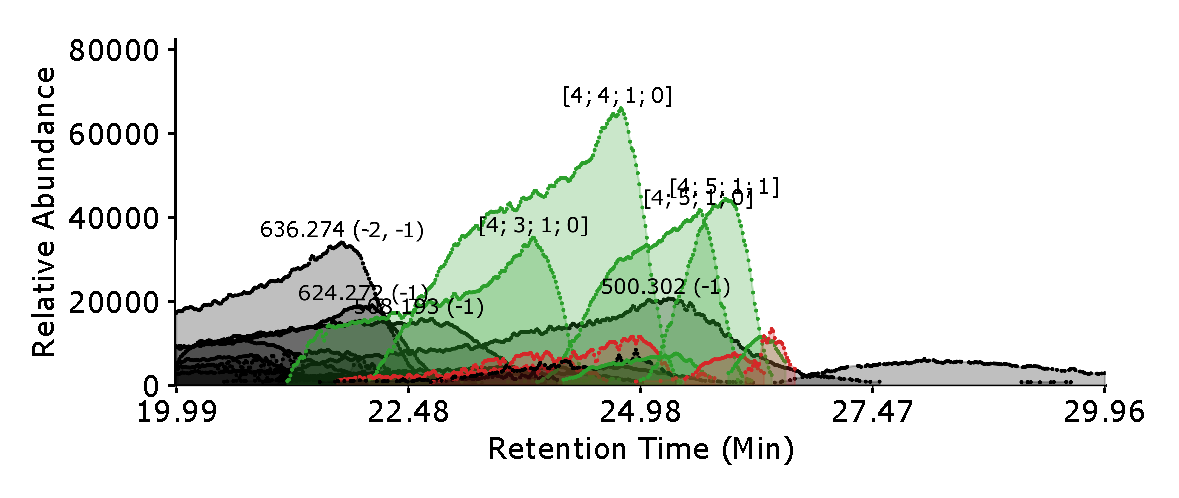
\includegraphics[width=1\linewidth, valign=t]{figure/native_igg_chromatograms.eps}
                \subcaption{
                    \label{fig:igg_assignment:a}
                }
            \end{subfigure}
            \vspace{0pt}
            \begin{subfigure}[b]{0.49\linewidth}
                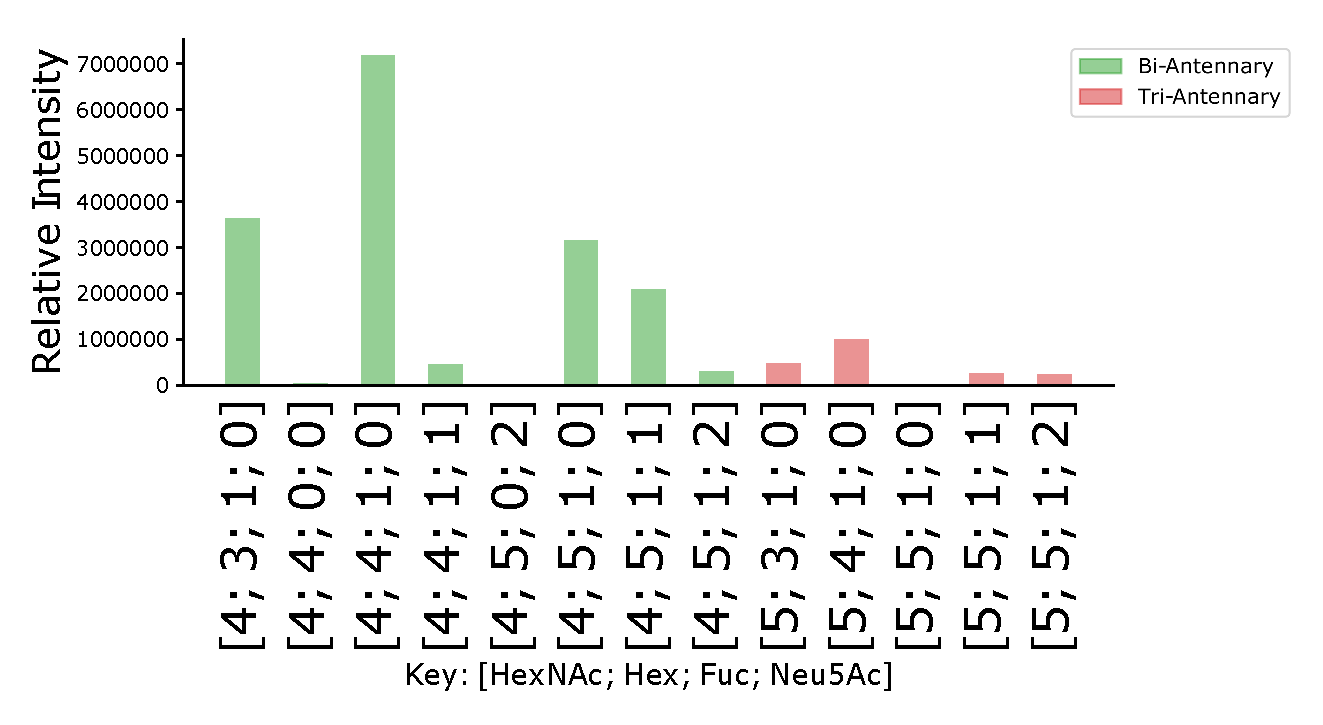
\includegraphics[width=1\linewidth, valign=b]{figure/native_igg_abundances.eps}
                \subcaption{
                    \label{fig:igg_assignment:b}
                }
            \end{subfigure}
        \end{minipage}
        \caption{Chromatogram Assignments for \igg
            \label{fig:igg_assignments}
        }
    \end{figure}


\section{Differences in Assigned Glycans for \rpserum}

    Of the compositions assigned by our algorithm that were not
    mentioned in \cite{Yu2013} but were annotated in the original publication
    of this dataset in \cite{Hu2012} include \textbf{HexNAc3 Hex4},
    \textbf{HexNAc3 Hex4 NeuAc1}, and \textbf{HexNAc5 Hex3}. Because our database
    was constructed based on combinatorial rules that did not take into account
    all biosynthetic constraints, we include infeasible compositions in our search
    space, such as \textbf{HexNAc2 Hex10 Fuc1} and \textbf{HexNAc5 Hex3 Fuc1 NeuAc2}.
    Future work could be done to restrict the database to only biosynthetically
    feasible glycan compositions. This would also have benefits for the construction
    of the composition network where only those compositions which have an enzymatic
    reaction to from one to the other would have an edge connecting them, such that
    \textbf{HexNAc5 Hex6 NeuAc2} would not have an edge to \textbf{HexNAc5 Hex7 NeuAc2}
    as in our current model.

\section{glySpace Integration and Upload}\label{sec:glyspace_integration_and_upload}

    We converted our \nglycan compositions into partially determined topologies
    assuming that the chitobios core was present to ensure that they were classified
    as \nglycans.

    From \rpserum
    \begin{verbatim}
        {Fuc:1; Hex:5; HexNAc:3; Neu5Ac:1}
        {Fuc:2; Hex:5; HexNAc:4; Neu5Ac:2}
        {Fuc:2; Hex:6; HexNAc:5; Neu5Ac:3}
        {Fuc:2; Hex:7; HexNAc:6; Neu5Ac:3}
        {Fuc:2; Hex:7; HexNAc:6; Neu5Ac:4}
        {Hex:7; HexNAc:6; Neu5Ac:2}
        {Hex:7; HexNAc:6; Neu5Ac:3}
        {Hex:8; HexNAc:7; Neu5Ac:3}
        {Hex:8; HexNAc:7; Neu5Ac:4}
        {Hex:9; HexNAc:8; Neu5Ac:2}
    \end{verbatim}

    From \philbs
    \begin{verbatim}
        {@sulfate:1; Fuc:1; Hex:4; HexNAc:5}
        {@sulfate:1; Fuc:1; Hex:5; HexNAc:4}
        {@sulfate:1; Fuc:1; Hex:5; HexNAc:5}
        {@sulfate:1; Fuc:2; Hex:4; HexNAc:5}
        {@sulfate:1; Fuc:2; Hex:6; HexNAc:5}
        {@sulfate:1; Fuc:2; Hex:9; HexNAc:8}
        {@sulfate:1; Fuc:3; Hex:4; HexNAc:5}
        {@sulfate:1; Fuc:3; Hex:6; HexNAc:5}
        {@sulfate:1; Fuc:3; Hex:9; HexNAc:8}
        {@sulfate:1; Fuc:4; Hex:6; HexNAc:5}
        {@sulfate:1; Fuc:4; Hex:8; HexNAc:7}
        {@sulfate:1; Fuc:4; Hex:9; HexNAc:8}
        {@sulfate:1; Hex:10; HexNAc:9}
        {@sulfate:1; Hex:4; HexNAc:5}
        {@sulfate:1; Hex:5; HexNAc:4}
        {Fuc:2; Hex:8; HexNAc:7}
        {Fuc:3; Hex:7; HexNAc:6}
        {Fuc:3; Hex:8; HexNAc:7}
        {Fuc:4; Hex:8; HexNAc:7}
        {Hex:10; HexNAc:9}
    \end{verbatim}

\bibliographystyle{natbib}
\bibliography{bibliography}

\end{document}
